\documentclass[11pt,a4paper,svgnames]{article}
\usepackage{babel}
\usepackage{fontspec}
\usepackage{luacode}
\usepackage{fancyhdr}
\usepackage{relsize}
%\usepackage[useregional]{datetime2}
%see https://tex.stackexchange.com/a/317859/42406
%\usepackage[utf8]{luainputenc}
%see https://tex.stackexchange.com/a/29594/42406
\usepackage{titling}
\usepackage[T1]{fontenc}
%\usepackage{xcolor}
\usepackage{hyperref}
%\usepackage{alltt}
%\usepackage{wasysym}
\usepackage{xcolor}
\usepackage{times}
%\usepackage[square]{natbib}
\usepackage{textcomp}
\usepackage{graphicx}
\usepackage{setspace}
\usepackage[backend=biber,bibencoding=utf8]{biblatex}
\addbibresource{../refpersys-bib.bib}
\usepackage[a4paper, margin=4cm]{geometry}
\setstretch{1.2}
\date{october 2019}
\newcommand*{\ac}[1]{\mbox{#1}}
\tolerance=600

\begin{luacode*}
  local gitpip=io.popen("git log --no-color --format=oneline -1 --abbrev=16 --abbrev-commit -q | cut -d' ' -f1")
  gitid=gitpip:read()
  gitpip:close()
  docdatetime = os.date('%Y-%b-%d %H:%M %Z')
  docdate = os.date('%Y-%b-%d')
\end{luacode*}
\newcommand{\mygitid}{\luadirect{tex.print(gitid)}}
\newcommand{\mydatetime}{\luadirect{tex.print(docdatetime)}}
\newcommand{\mydate}{\luadirect{tex.print(docdate)}}
\newcommand{\RefPerSys}{{\textit{\textsc{RefPerSys}}}}

 % see https://tex.stackexchange.com/a/51349/42406
\hypersetup{
  colorlinks   = true, %Colours links instead of ugly boxes
  urlcolor     = NavyBlue, %Colour for external hyperlinks
  linkcolor    = DarkGreen, %Colour of internal links
  citecolor   = DarkMagenta, %Colour of citations
  frenchlinks = true,
}
\setlength{\droptitle}{-10em}   % This is your set screw

\pagestyle{fancy}
\fancyhf{}
\rhead{\textit{\textsc{RefPerSys}} high-level goals and design ideas}
\fancyfoot[L]{{\raisebox{0.0cm}[1pt][1pt]{\color{LightSlateGrey}{{\relsize{+1}{DRAFT}}}~\relsize{-1.5}{\texttt{\mygitid} on \textit{\mydate}}}}}
\fancyfoot[R]{{Page \thepage}}
\begin{document}
\title {\textit{\textsc{RefPerSys}} high-level goals and design
  ideas\thanks{This document has git commit \texttt{\mygitid},
    was Lua-{\LaTeX} generated on \textit{\mydatetime}, see
    \href{http://gitlab.com/bstarynk/refpersys}{\texttt{gitlab.com/bstarynk/refpersys/}}
    and its \texttt{doc/design-ideas} subdirectory. Its draft is downloadable, as a \href{https://en.wikipedia.org/wiki/PDF}{PDF} file, from \href{http://starynkevitch.net/Basile/refpersys-design.pdf}{\texttt{starynkevitch.net/Basile/refpersys-design.pdf}} \ldots}}
\author {Basile
  \textsc{Starynkevitch}\thanks{See
    \href{http://starynkevitch.net/Basile/}{\texttt{starynkevitch.net/Basile/}}
    and contact
    \href{mailto:basile@starynkevitch.net}{\texttt{basile@starynkevitch.net}},
    92340 Bourg La Reine {\relsize{-1}(near Paris)}, France.}}

\begin{titlepage}
  \thispagestyle{empty}
  \maketitle

  \bigskip

  \begin{abstract}
    \textit{\textsc{RefPerSys}} is a \textsc{\textbf{Ref}}lexive and
    orthogonally \textsc{\textbf{Per}}sistent \textsc{\textbf{Sys}}tem
    (as a GPLv3+ licensed free software\footnote{Some code is
    available on
    \href{https://gitlab.com/bstarynk/refpersys}{\texttt{gitlab.com/bstarynk/refpersys}}.})
    running on Linux; it is a hobby but serious \textbf{research
      project} for many years, mostly aimed to experiment \textbf{open
      science} ideas close to
    {AGI}\footnote{{\href{https://en.wikipedia.org/wiki/Artificial\_general\_intelligence}{Artificial
        General Intelligence}}} dreams, and we don't expect useful or
    interesting results before several years of hard work.
  \end{abstract}

  \medskip

  \textbf{audience :} \textsc{Linux} free software
  developers\footnote{Those \textsc{Linux} software developers are
  routinely \emph{glancing inside}, \emph{building} then using -from
  their published source code- quite large open source programs (such
  as \href{http://gcc.gnu.org/}{\textsc{Gcc}},
  \href{http://sbcl.org/}{\textsc{Sbcl}},
  \href{https://www.call-cc.org/}{\textsc{Chicken-Scheme}},
  \href{http://hop.inria.fr/}{\textsc{Hop}},
  \href{https://haxe.org/}{\textsc{Haxe}},
  \href{https://ocsigen.org}{\textsc{Ocsigen}},
  \href{https://www.gnu.org/software/emacs/}{\textsc{Emacs}},
  \href{https://sqlite.org/}{\textsc{Sqlite}},
  \href{https://mariadb.org/}{\textsc{MariaDb}}, etc...)  and perhaps
  even contributing to smaller free software projects like
  \href{https://ninja-build.org/}{\textsc{Ninja}},
  \href{https://github.com/davidmoreno/onion}{\texttt{libonion}},
  etc... By the way, all these open source projects could be useful to
  or inspirational for \RefPerSys.} and computer scientists interested in
  an experimental open science approach to reflexive systems,
  orthogonal persistency, symbolic artificial intelligence, knowledge
  engines, etc....


  \medskip
  \textbf{Nota Bene:} this report contains
  \href{https://en.wikipedia.org/wiki/Hyperlink}{hyperlinks} so its
  \href{https://en.wikipedia.org/wiki/PDF}{PDF} should rather be read
  on a computer screen, e.g. with
  \href{https://en.wikipedia.org/wiki/Evince}{\texttt{evince}}. Since
  it describes a circular design (with many
  \href{https://en.wikipedia.org/wiki/Cycle_graph}{cycles}
  \cite{Hofstadter:1979:GEB}), we recommend to read it twice (skipping
  footnotes and references on the first read).

  \bigskip


  \begin{quote}
  \begin{relsize}{-1}
  \includegraphics[width=75pt]{CC-BY-SA-icon} This entire document is
  licensed under the Creative Commons Attribution-ShareAlike 4.0
  International License. To view a copy of this license, visit
  \href{http://creativecommons.org/licenses/by-sa/4.0/}{\texttt{creativecommons.org/licenses/by-sa/4.0/}}
  or send a letter to Creative Commons, PO Box 1866, Mountain View, CA
  94042, USA.
  \end{relsize}
  \end{quote}
  
\end{titlepage}



\tableofcontents

\bigskip


\section{\textsc{RefPerSys} ambitions and goals}
\label{sec:ambitions-goals}

The \RefPerSys\footnote{For a \textbf{Ref}lexive \textbf{Per}sistent
  \textbf{Sys}tem}~ system shares several -but not all- goals and
design ideas (but no code) with
\href{http://github.com/bstarynk/bismon}{\texttt{bismon}}
\cite{Starynkevitch:2019:bismon-draft} but of course \emph{not}
\texttt{bismon}'s application\footnote{I Basile am not allowed and not
  funded to directly work on
  \href{https://en.wikipedia.org/wiki/Artificial_general_intelligence}{AGI}
  -which still is my major personal scientific interest- but I do get
  funded on applied research projects like
  \href{https://www.decoder-project.eu/}{\textsc{Decoder}} and try to
  push some AGI ideas into them.} to
\href{https://en.wikipedia.org/wiki/Static_program_analysis}{static
  source code analysis}. Like \texttt{bismon}, {\RefPerSys} is a
\textbf{reflexive} (it uses
\href{https://en.wikipedia.org/wiki/Reflection_(computer_programming)}{reflection}),
\textbf{\href{https://en.wikipedia.org/wiki/Virtual\_machine\_introspection}{introspective}}
and \textbf{orthogonally
  \href{https://en.wikipedia.org/wiki/Persistence_(computer_science)}{persistent}}
system, but not for
\href{https://en.wikipedia.org/wiki/Static_program_analysis}{static
  program analysis}. Please read Bismon's draft report
\cite{Starynkevitch:2019:bismon-draft} for a more precise definition
of these concepts. \textbf{\RefPerSys~ is a long term\footnote{I don't
    expect any significant AGI research results before $\approx
    2026$.}  risky
  \href{https://en.wikipedia.org/wiki/Research}{research} project with
  an \href{https://en.wikipedia.org/wiki/Open_science}{open science}
  mindset and
  \href{https://ropensci.github.io/reproducibility-guide/sections/introduction/}{reproducible
    experiment} ethics \cite{zuboff:2015:big-other,
    oneil:2016:weapons}, and a
  \href{https://www.gnu.org/philosophy/free-sw.en.html}{free software}
  licensed under
  \href{https://www.gnu.org/licenses/gpl-3.0.html}{GPLv3+}, and
  targetted \emph{only} for \textsc{Linux x86-64} computers.}. A Linux
system\footnote{My own \texttt{ours.starynkevitch.net} computer,
  running \textit{Debian/Unstable}, has 64 Gibytes of RAM, 24 cores
  (AMD 2970WX) and terabytes of disk space, including a terabyte of
  SSD.}  with at least 16 Gibytes of RAM, 4 \textit{x86-64} cores, and
220 Gibytes of disk is required. The grand ambition of {\RefPerSys} is
to become later an infrastructure for some strong
\href{https://en.wikipedia.org/wiki/Artificial_general_intelligence}{AGI}
system à la \textsc{Caia}\footnote{With explicit permission from
  J.Pitrat, \textsc{Caia} source code -entirely generated by itself,
  about half a million lines of C code- is available on
  \href{http://starynkevitch.net/Basile/}{my (Basile's) web page} as
  \href{http://starynkevitch.net/Basile/caia-su-24feb2016.tar.bz2}{\texttt{caia-su-24feb2016.tar.bz2}},
  and you could build it with \texttt{gcc -O -g [A-Z]*.c -rdynamic
    -ldl} then run \texttt{./a.out}. However, since I Basile sadly
  failed to convince J.Pitrat that open source
  \cite{Lerner-Tirole:2000:economics-open-source,
    Weber:2004:SuccessOpenSource} software are -in our
  XXI\textsuperscript{th} century- also an important way to transmit
  research ideas, there are no complete instructions to use it. Hence
  \textsc{Caia} has an undocumented user interface as user-friendly as
  the one of \href{https://www.gnu.org/software/ed/}{\texttt{ed}} but
  convenient enough to J.Pitrat alone! If you are capable of reading
  some comments in French and guessing the semantics of declarative
  ``expert system'' like rules (\textsc{Caia} has more than a dozen of
  thousands of them), run it, then type \texttt{L EDITE} and start
  reverse-engineering that brillant \textsc{Caia} system.}  by Jacques
Pitrat\footnote{Jacques Pitrat has passed away on October
  14\textsuperscript{th}, 2019. See quickly also his old web page on
  \href{http://jacques.pitrat.pagesperso-orange.fr/}{\texttt{jacques.pitrat.pagesperso-orange.fr}}
  and his interesting blog on
  \href{http://bootstrappingartificialintelligence.fr/WordPress3/}{\texttt{bootstrappingartificialintelligence.fr/WordPress3}}
  \ldots} \cite{Pitrat:1996:FGCS, Pitrat:2009:AST,
  Pitrat:2009:ArtifBeings}, but before even approaching that goal a
big lot of work is required, and {\RefPerSys} should be valuable by
itself for other less ambitious and more pragmatical purposes, perhaps
some specialized collaborative web server (GPLv3+) to ease
communication between human {\RefPerSys} developers, that is a mix of
a wiki, a chat, and a tool for sharing document with drawings or
graphics.

The development of {\RefPerSys} is (like the one of \texttt{bismon},
or
\href{http://bootstrappingartificialintelligence.fr/WordPress3/?s=CAIA}{of
  \textsc{Caia}}) a slow, incremental and gradual
\href{https://en.wikipedia.org/wiki/Bootstrapping}{bootstrapping}
process with a meta-programming \cite{dormoy:1992:meta} approach :
features added to {\RefPerSys} in January 2020 are used to implement
new features worked on a later {\RefPerSys} in March 2020.

As every practical software, {\RefPerSys} targets some defined
machines: common Linux distribution running on some
computer\footnote{For several years, that computer is a desktop or
powerful laptop running some \textsc{Debian}. Later that could be some
``virtual machine'' e.g. some
\href{https://www.docker.com/}{\textsc{Docker}} container.}. So the
target machine of {\RefPerSys} is a quite complete and modern Linux
system (such as a recent \textit{\textsc{Debian}} or
\textit{\textsc{Ubuntu}} desktop), with many useful packages, and
administred by some human person\footnote{For obvious cybersecurity
reasons, automatic administration of that Linux distribution is out of
scope. Also, since Basile Starynkevitch is still working (in october
2019) in a cybersecurity
\href{http://www-list.cea.fr/en/technological-research/research-programmes/embedded-systems/validation-and-verification}{lab}
(of about 25 permanent staff) at
\href{http://www-list.cea.fr/}{CEA/LIST}, cybersecurity concerns would
be a conflict of interest.}. The {\RefPerSys} system is published in
``source'' form, as a set of \href{http://git-scm.com/}{\texttt{git}}
versioned\footnote{We crucially depend upon \texttt{git}
\emph{specifically} (e.g. \href{http://gitlab.org/}{\texttt{gitlab}}),
and \href{https://en.wikipedia.org/wiki/Porting}{porting} {\RefPerSys}
to some other versioning system -or to some other
\href{http://pages.cs.wisc.edu/~remzi/OSTEP/}{operating system} than
\textsc{Linux}- would be a quite difficult task.} textual files
(e.g. \textit{C++} or \textit{C} files\footnote{However, notice that
bootstrapped language implementations like
\href{http://s48.org/}{Scheme 48} or \href{https://ocaml.org/}{Ocaml}
are keeping some
\href{https://en.wikipedia.org/wiki/Bytecode}{bytecode} form under
version control, and \href{https://www.call-cc.org/}{\textsc{Chicken
    Scheme}} is, like \texttt{bismon}, \texttt{git}-keeping generated
C files.}, perhaps some
\href{https://en.wikipedia.org/wiki/Makefile}{\texttt{Makefile}} or
better yet an
\href{http://projects.camlcity.org/projects/omake.html}{\textsc{Omake}}
build -most and more and more\footnote{Of course, in a
\href{https://en.wikipedia.org/wiki/Chicken_or_the_egg}{chicken and
  egg} fashion, the initial version of {\RefPerSys} has to contain
mostly hand-written files!} of them being generated- or shell files or
data files). Some of these files are generated, and the bootstrapping
goal is to have \emph{every} \texttt{git}-registered textual file been
generated by {\RefPerSys}, with a
\href{https://en.wikipedia.org/wiki/Bootstrapping\_(compilers)}{\textbf{bootstrap}ed}
approach\footnote{Observe that Linux source distributions like \href{http://www.linuxfromscratch.org/}{\texttt{linuxfromscratch.org}}, or to a lesser extent \href{https://www.gentoo.org/}{GenToo}, are also, when considered as a single system, fully bootstrapped.} similar to those of
\href{https://en.wikipedia.org/wiki/Self-hosting_(compilers)}{self-hosting
  compilers}.
\medskip

Within {\RefPerSys}, we call\footnote{Notice that, on purpose, our
terminology is different of usual habits in the open source realm:
almost all software projects (see also
\href{http://softwareheritage.org}{\texttt{softwareheritage.org}}) are
made of
\href{https://en.wikipedia.org/wiki/Computer\_file}{\textit{computer
    files}} typed by human developers in some
\href{https://en.wikipedia.org/wiki/Source-code\_editor}{source-code
  editor} or some
\href{https://en.wikipedia.org/wiki/Integrated\_development\_environment}{IDE}
such as \href{https://www.gnu.org/software/emacs/}{\texttt{emacs}},
\href{http://vim.org/}{\texttt{vim}} or
\href{http://codeblocks.org/}{\texttt{Code::Blocks}}, according to the
old \href{https://en.wikipedia.org/wiki/Unix\_philosophy}{Unix
  philosophy}. Notice that large open source projects like the
\href{https://www.libreoffice.org/}{\textsc{LibreOffice}} suite, the
\href{http://gcc.gnu.org}{\textsc{Gcc}} compiler collection or the
\href{https://www.mozilla.org/en-US/firefox/}{FireFox} browser tend to
accept
\href{https://en.wikipedia.org/wiki/Plug-in_(computing)}{plugins}
instead of favoring old fashioned
\href{https://en.wikipedia.org/wiki/Pipeline_(Unix)}{command
  pipelines}, but multi-threaded applications may follow the
\href{https://en.wikipedia.org/wiki/Pipeline_(software)}{pipeline
  design pattern}. In contrast, we are impatient to reach the state
where all {\RefPerSys} source files have been \texttt{git}-versioned
but are all generated by a previous run of our \texttt{refpersys}
executable. The {\RefPerSys} developer is interacting, thru a web
interface, with some running \texttt{refpersys} process, which is also some
specialized web server (using  HTTP).}  ``source file'' any Linux file which is
\texttt{git}-versioned. We hope that more and more of these source
files will be generated by the \texttt{refpersys}
\href{https://en.wikipedia.org/wiki/Executable\_and\_Linkable_Format}{ELF}
\href{https://en.wikipedia.org/wiki/Executable}{executable}
program. \textbf{A significant milestone is the entire bootstrapping
  of \RefPerSys}, when all files (in textual form, to stay
\texttt{git}-friendly, like
\href{https://en.wikipedia.org/wiki/Text-based_protocol}{text based
  protocols} are more friendly for developers) can be regenerated by
the \texttt{refpersys} executable, exactly in the same state as they
were previously\footnote{Pedantically, some
\href{https://en.wikipedia.org/wiki/Fixed\_point\_(mathematics)}{fixpoint}
of some very coarse-grained
\href{https://en.wikipedia.org/wiki/Operational\_semantics}{operational
  semantics} related to
\href{https://en.wikipedia.org/wiki/Abstract\_interpretation}{abstract
  interpretation} and
\href{https://en.wikipedia.org/wiki/Operational\_semantics\#Structural\_operational\_semantics}{big
  step semantics}, each big step being the entire regeneration of the
system, inspired by Futurama projections and
\href{https://en.wikipedia.org/wiki/Partial\_evaluation}{partial
  evaluation}.} : as a whole, our {\RefPerSys} system should become a
\href{https://en.wikipedia.org/wiki/Quine\_(computing)}{Quine
  program}, and \textsc{Caia} is already one. So the
\href{https://en.wikipedia.org/wiki/Build\_automation}{build
  automation} tool which compiles {\RefPerSys} should use file
contents, not modification times to trigger compilation commands,
since a full regeneration of such a bootstrapped {\RefPerSys} system
will touch all files, without changing the content of any of
them. Hence and very concretely, for building {\RefPerSys} the
\href{http://projects.camlcity.org/projects/omake.html}{\texttt{omake}}
build automation tool is preferable to \textsc{Gnu}
\href{https://www.gnu.org/software/make/}{\texttt{make}}.

For pragmatical reasons, \textbf{{\RefPerSys} needs a good
  \href{https://en.wikipedia.org/wiki/Tracing\_garbage\_collection}{garbage
    collector}} (or GC \cite{jones:2016:gchandbook}), since fully
compile-time GC \cite{mazur:2004:compile} are too difficult to
implement. Since multi-core x86-64 machines are very common, it should
take advantage of them, so \textbf{{\RefPerSys} should follow a
  \href{https://en.wikipedia.org/wiki/Thread_(computing)}{multi-threaded}
  approach} above \textsc{Posix} \cite{barney:2010:pthreads} or
\href{https://en.cppreference.com/w/cpp/thread}{C++11 threads}. Our GC
should be a
\href{https://en.wikipedia.org/wiki/Tracing_garbage_collection#Precise_vs._conservative_and_internal_pointers}{precise}
garbage collector \cite{Rafkind:2009:PreciseGC} and we may want to
favor, like what was done in \textsc{Gcc Melt}
\cite{Starynkevitch:2007:Multistage, Starynkevitch-DSL2011,
  Starynkevitch-GCCMELTweb}, fast allocation of small memory zones
which get quickly disposed of when becoming dead using a copying
generational
\href{https://en.wikipedia.org/wiki/Cheney's\_algorithm}{Cheney-like
  GC algorithm} \cite{wilson:1992:uniprocessorgc}.  But mixing
precise, sometimes generational GC techniques with multi-threading is
a difficult programming task. But precise-GC friendly programming is
simpler in generated C or C++ code that with hand-written code
(because of explicit management of local GC roots and write barriers,
à la
\href{http://starynkevitch.net/Basile/qishintro.html}{\textsc{Qish}}
or
\href{https://caml.inria.fr/pub/docs/manual-ocaml/intfc.html}{\textsc{Ocaml}}:
garbage collection invariants are boring and brittle to maintain in
hand-written code).


\href{https://en.wikipedia.org/wiki/Reification_(computer_science)}{Reification}
is an important concept in \RefPerSys, including (later) at the
\href{https://en.wikipedia.org/wiki/Knowledge_representation_and_reasoning}{knowledge
  representation} level with
\href{https://en.wikipedia.org/wiki/Semantic_network}{semantic
  networks} and
\href{https://en.wikipedia.org/wiki/Frame_(artificial_intelligence)}{frames}. {\RefPerSys}
\href{https://en.wikipedia.org/wiki/Call_stack}{call stacks} are made
of call frames known to our garbage collector (like
\href{https://caml.inria.fr/pub/docs/manual-ocaml/intfc.html}{\textsc{Ocaml}}'s
ones). They could later be copied into data structures representing
some
\href{https://en.wikipedia.org/wiki/Delimited_continuation}{delimited
  continuations} \cite{Reynolds:1993:continuations,
  Queinnec:2004:ContinWeb}, perhaps even representing and describing
control \cite{fouet-starynkevitch:describing-control:1987,
  Starynkevitch-1990-EUM, Pitrat:2009:ArtifBeings}. This should also
enable \textbf{introspection}, by permitting primitives inspecting the
current call stack, perhaps using Ian Taylor's
\href{https://github.com/ianlancetaylor/libbacktrace}{\texttt{libbacktrace}}.


{\RefPerSys} should (like \textsc{Caia} and its predecessor
\textsc{Malice} did
\cite{Pitrat:2009:AST,Pitrat:1996:FGCS,Pitrat:2009:ArtifBeings}) have
some expert system shell \cite{kumar:2015:importance-expert-systems,
  nigro:2008:meta} and meta-rules to ``dynamically compile'' some
subset of expert system rules and knowledge bases to procedural code
(e.g. with a metaprogramming approach of generating \emph{C} code, or
\href{https://gcc.gnu.org/onlinedocs/jit/}{\texttt{libgccjit}}
compiled code, then
\href{http://man7.org/linux/man-pages/man3/dlopen.3.html}{\texttt{dlopen(3)}}-ing
that code and running it at runtime. The
\href{https://github.com/bstarynk/misc-basile/blob/master/manydl.c}{\texttt{manydl.c}}
program show that this can practically be done many dozen of thousands
of times on Linux desktops).


Most Linux distributions contain lots of useful libraries or software
components for {\RefPerSys} long-term goals, notably machine learning
open source libraries like
\href{https://www.tensorflow.org/}{\textsc{TensorFlow}}
\cite{charniak:2019:deep-learning} or
\href{https://gudhi.inria.fr/}{\textsc{Gudhi}}
\cite{chazal:2016:high}. We don't want to rewrite them inside
\RefPerSys. Hence, we will need in {\RefPerSys} to generate some glue
code, like \href{http://swig.org/}{\textsc{Swig}} does, from some
declarative description (probably some frames or knowledge bases) of
the
\href{https://en.wikipedia.org/wiki/Application_programming_interface}{API}
of these available libraries.


\subsection{{\RefPerSys} strange development cycle}
\label{subsec:strange-devel}

Ordinary software projects tend to follow a spiral development model
\cite{boehm:1988:spiral} as shown in figure \ref{fig:tradspiral}.

\begin{figure}[h]
  \begin{center}
    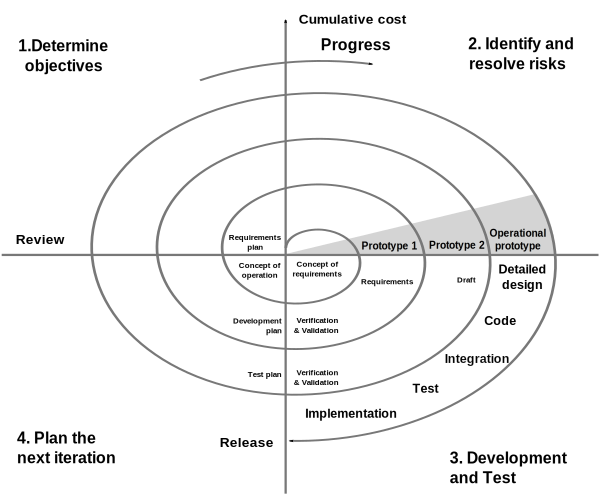
\includegraphics[width=0.8\textwidth]{spiral-model-softdevel}
  \end{center}
  \caption{the traditional spiral development model (from Wikipedia \href{https://en.wikipedia.org/wiki/Spiral_model}{spiral model})}
  \label{fig:tradspiral}
\end{figure}

But \RefPerSys' development follows a strange loop
\cite{hofstadter:2007:strange-loop}, since it is bootstrapped in an \href{https://en.wikipedia.org/wiki/Software\_prototyping\#Evolutionary\_prototyping}{evolutionary prototyping} manner. It is more like a spiral staircase 

\begin{figure}[h]
  \begin{center}
    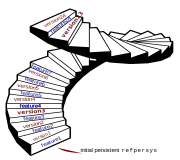
\includegraphics[width=0.8\textwidth]{spiral-stairs}
  \end{center}
  \caption{the {\RefPerSys} staircase development model {\relsize{-1}{(from a \href{https://thenounproject.com/term/spiral-stairs/956427/}{figure of Spiral stairs} by Lluisa Iborra from the Noun Project)}}}
  \label{fig:bootstrap-stair}
\end{figure}

\clearpage


\printbibliography

\end{document}

%%%%%%%%%%%%%%%%%%%%%%%%%%%%%%%%%%%%%%%%%%%%%%%%%%%%%%%%%%%%%%%%
%% Local Variables: ;;
%% compile-command: "./build.sh" ;;
%% End: ;;
%%%%%%%%%%%%%%%%%%%%%%%%%%%%%%%%%%%%%%%%%%%%%%%%%%%%%%%%%%%%%%%%
